\chapter{Tinjauan Pustaka}

\section{Penelitian Terdahulu}

\cite{kratica2007} mengkaji pendekatan heuristik berbasis \foreign{genetic algorithm} untuk menghitung dimensi metrik pada berbagai kelas graf. Algoritma yang diusulkan menggunakan representasi biner, teknik \foreign{frozen-gene mutation}, serta mekanisme \foreign{caching} untuk meningkatkan efisiensi pencarian. Hasil utama yang diperoleh adalah: 1) algoritma mampu menemukan dimensi metrik untuk graf berukuran besar yang sulit ditangani secara analitik; 2) solusi yang diperoleh mendekati nilai optimal yang sudah diketahui pada berbagai contoh graf; serta 3) eksperimen menunjukkan bahwa pendekatan ini lebih unggul dibandingkan metode heuristik sederhana. Penelitian ini menunjukkan bahwa metode metaheuristik dapat digunakan secara efektif untuk menghampiri perhitungan dimensi metrik pada graf kompleks.

\cite{eppstein2015} meneliti dimensi metrik dari perspektif kompleksitas terparameter dengan menggunakan parameter \textit{max leaf number}. Hasil utama yang diperoleh adalah: 1) pembuktian bahwa dimensi metrik bersifat \foreign{fixed-parameter tractable} (FPT) jika diparameterkan oleh \textit{max leaf number}; 2) perancangan algoritma dengan waktu komputasi \(O(n) + 2^{O(\ell^{6} \log \ell)} \log n\), di mana \(\ell\) adalah \textit{max leaf number} dari graf; serta 3) identifikasi bahwa meskipun algoritma ini belum praktis karena kompleksitas eksponensial, pendekatan ini membuka jalan untuk kemungkinan reduksi kompleksitas lebih lanjut atau penggunaan parameter lain, seperti \textit{cyclomatic number}. Penelitian ini memperluas kajian algoritmik dimensi metrik dengan menempatkannya dalam kerangka teori kompleksitas terparameter.

\cite{kelenc2018} memperkenalkan dan mengkaji konsep dimensi metrik sisi pada graf, yaitu banyak minimum simpul yang dapat membedakan setiap pasangan sisi. Mereka menunjukkan bahwa parameter ini memenuhi sifat-sifat dasar yang mirip dengan dimensi metrik. Beberapa hasil utama yang diperoleh adalah: 1) pembuktian bahwa menentukan dimensi metrik sisi bersifat \foreign{NP-hard}; 2) penentuan dimensi metrik sisi untuk berbagai kelas graf khusus, termasuk graf lintasan, graf melingkar, dan graf roda; 3) penyelidikan hubungan antara dimensi metrik sisi dan parameter graf lainnya. Penelitian ini memberikan landasan teoretis awal untuk studi lebih lanjut mengenai dimensi metrik sisi.

\cite{klavzar2020} mengkaji dimensi metrik sisi pada graf melalui dua pendekatan, yaitu analisis produk hierarkis dan formulasi \foreign{integer linear programming} (ILP). Hasil utama yang diperoleh adalah: 1) penentuan batas atas untuk dimensi metrik sisi dari produk hierarkis \(G(U) \,\widehat{\times}\, H\), serta formula eksak pada kasus \(|U| = 1\); 2) pengembangan model ILP untuk menghitung dimensi metrik sisi secara komputasional; 3) penerapan metode tersebut pada berbagai graf dari kimia matematika, termasuk graf molekul dan fullerene, yang menunjukkan efektivitas model dalam memberikan solusi tepat. Penelitian ini memperluas studi dimensi metrik sisi dengan menggabungkan hasil teoritis dan pendekatan optimisasi komputasional.

\cite{knor2021} meneliti hubungan antara dimensi metrik dan dimensi metrik sisi. Penelitian ini menyelesaikan tiga permasalahan terbuka mengenai dimensi tersebut. Hasil utama yang diperoleh adalah: 1) untuk setiap bilangan bulat \(r\), \(t \geq 2\) dengan \(r \neq t\), terdapat graf berorde \(n\) cukup besar sehingga memiliki dimensi metrik \(r\) dan dimensi metrik sisi \(t\); 2) terbukti bahwa rasio antara dimensi metrik dan dimensi metrik sisi tidak terbatas dari atas; 3) ditemukan adanya keluarga graf tak hingga yang memiliki dimensi metrik sisi lebih kecil daripada dimensi metrik. Selain itu, mereka juga mengidentifikasi graf terkecil (berorde 10 dan 11) yang memenuhi kondisi tersebut. Temuan ini menunjukkan bahwa hubungan antara kedua parameter tersebut tidak dapat dibatasi dengan faktor konstan tertentu.

Berdasarkan penelitian-penelitian terdahulu, dapat dilihat bahwa kajian mengenai dimensi metrik dan dimensi metrik sisi pada graf telah berkembang melalui berbagai pendekatan, mulai dari pengembangan teori dasar, pembuktian sifat-sifat struktural, formulasi optimisasi, hingga metode heuristik dan metaheuristik. Namun, sebagian besar penelitian tersebut masih berfokus pada pendekatan analitik maupun algoritmik konvensional. Belum terdapat penelitian yang secara khusus memanfaatkan formulasi ke dalam \foreign{Satisfiability Modulo Theories} (SMT) sebagai alternatif untuk memodelkan dan menyelesaikan permasalahan ini. Oleh karena itu, tugas akhir ini hadir untuk mengisi celah tersebut dengan merepresentasikan permasalahan dimensi metrik dan dimensi metrik sisi ke dalam formula SMT serta menguji efektivitas \foreign{solver} SMT, dalam menghitung nilai kedua parameter tersebut.

\section{Graf}

Graf adalah struktur yang terdiri dari himpunan simpul dan himpunan sisi, yang setiap sisinya menghubungkan sepasang simpul dalam himpunan simpul tersebut \citep{harary1969}. Misalkan sebuah graf memiliki 5 simpul \(V = \{x_1, x_2, x_3, x_4, x_5\}\) dan 8 sisi \(E = \{e_1, e_2, e_3, e_4, e_5, e_6, e_7, e_8\}\). Setiap sisi tersebut berturut-turut menghubungkan pasangan simpul \((x_1, x_3)\), \((x_1, x_4)\), \((x_1, x_5)\), \((x_2, x_4)\), \((x_2, x_5)\), \((x_3, x_4)\), \((x_3, x_5)\), dan \((x_4, x_5)\). \autoref{fig:contoh-graf} menunjukkan graf ini.

Lintasan adalah rangkaian sisi yang menghubungkan rangkaian simpul, dengan setiap ujung sisinya merupakan simpul berurutan \citep{west1996}. Contohnya, pada \autoref{fig:contoh-graf}, \((x_2, x_4, x_3, x_1)\) adalah lintasan, karena dapat dihubungkan dengan rangkaian \((e_4, e_6, e_1)\). Sedangkan \((x_5, x_2, x_3)\) bukanlah lintasan, karena tidak terdapat sisi yang menghubungkan simpul \(x_2\) dan \(x_3\). Lintasan dengan ujung simpul \(v, w\) disebut sebagai lintasan yang menghubungkan \(v\) dan \(w\). Pada suatu graf, bisa terdapat banyak lintasan yang menghubungkan sepasang simpul \citep{west1996}. Sehingga, lintasan \((e_4, e_6, e_1\)) disebut menghubungkan \(x_2\) dan \(x_1\).

\noindent
\begin{center}
	\begin{minipage}{0.4\linewidth}
		\centering
		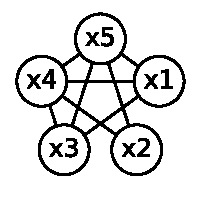
\includegraphics[width=0.625\linewidth]{img/8ec60eeeaa549478379fc4cb6b42df17c5ca8b364e4e642efbba0ac2db0b6e94.pdf}
		\vspace{-1em}
		\captionof{figure}{\centering Graf Terhubung}
		\label{fig:contoh-graf}
	\end{minipage}
	\begin{minipage}{0.4\linewidth}
		\centering
		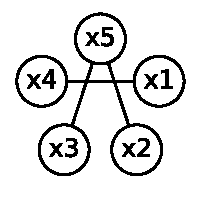
\includegraphics[width=0.625\linewidth]{img/0630ebfe671b8208b2dc56ca90c62464252c4ac5e3f30ff3fc2c6db4495f49cc.pdf}
		\vspace{-1em}
		\captionof{figure}{\centering Graf Tak Terhubung}
		\label{fig:graf-tak-terhubung}
	\end{minipage}
\end{center}

Graf terhubung adalah graf dengan setiap pasang simpulnya memiliki lintasan yang menghubungkan \citep{chartrand2000}. \autoref{fig:contoh-graf} adalah contoh graf terhubung. \autoref{fig:graf-tak-terhubung} adalah contoh graf tak terhubung karena tidak terdapat lintasan yang dapat menghubungkan \(x_1\) dan \(x_5\).

Jarak antara dua simpul \(u\) dan \(v\), dinotasikan \(d(u, v)\), adalah panjang minimum dari semua lintasan yang menghubungkan kedua simpul tersebut \citep{chartrand2000}. Panjang sebuah lintasan adalah banyaknya sisi yang membangun rangkaian lintasan tersebut. Contoh, pada \autoref{fig:contoh-graf}, nilai dari \(d(x_2, x_1)\) adalah \(2\).

Matriks ketetanggaan adalah alternatif representasi dari graf yang menunjukkan ketetanggaan, atau keberadaan sisi antar simpul \citep{west1996}. Semisalnya sebuah graf memiliki himpunan simpul \(V = \{v_1, v_2, \ldots\}\). Maka, baris dan kolom pertama dalam matriks ketetanggaannya menunjukkan \(v_1\), baris dan kolom kedua menunjukkan \(v_2\), dan seterusnya. Ketika terdapat sisi yang menghubungkan \(v_i\) ke \(v_j\), maka elemen pada baris ke-\(i\) dan kolom ke-\(j\) bernilai \(1\), sedangkan bila tidak terhubung maka bernilai \(0\). Sebagai ilustrasi, berikut adalah matriks ketetanggaan dari \autoref{fig:contoh-graf}.
\[
\left[
\begin{array}{ccccc}
	0 & 0 & 1 & 1 & 1 \\
	0 & 0 & 0 & 1 & 1 \\
	1 & 0 & 0 & 1 & 1 \\
	1 & 1 & 1 & 0 & 1 \\
	1 & 1 & 1 & 1 & 0
\end{array}
\right]
\]
Perhatikan matriks ketetanggaan simetris terhadap diagonal utama ketika graf yang direpresentasikan tak berarah.

Matriks jarak adalah matriks yang memuat jarak antara seluruh pasangan simpul \citep{chartrand2000}. Sehingga, setiap baris ke-\(i\) dan kolom ke-\(j\) berisi nilai jarak dari \(v_i\) ke \(v_j\), seperti berikut:
\[
\left[
\begin{array}{ccc}
	d(v_1, v_1) & d(v_1, v_2) & \cdots \\
	d(v_2, v_1) & d(v_2, v_2) & \cdots \\
	\vdots & \vdots & \ddots
\end{array}
\right]
\]
Dan sebagai gambaran, berikut adalah matriks jarak dari \autoref{fig:contoh-graf}.
\[
\left[
\begin{array}{ccccc}
	0 & 2 & 1 & 1 & 1 \\
	2 & 0 & 2 & 1 & 1 \\
	1 & 2 & 0 & 1 & 1 \\
	1 & 1 & 1 & 0 & 1 \\
	1 & 1 & 1 & 1 & 0
\end{array}
\right]
\]
Dapat diamati, setiap elemen dalam matriks jarak memiliki nilai ketika graf yang direpresentasikan adalah graf terhubung.

\section{Automorfisma Graf}

\noindent
\begin{center}
	\begin{minipage}{0.8\linewidth}
		\begin{minipage}{0.25\linewidth}
			\centering
			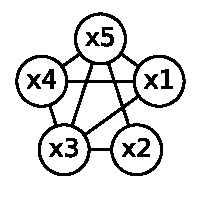
\includegraphics[width=\linewidth]{img/3637d326d230653eb5359219776827aba655cda549265e8622f29fcf4522cfb1.pdf}
			\vspace{-2em}
			\par\small (a)
		\end{minipage}
		\hfill
		\begin{minipage}{0.25\linewidth}
			\centering
			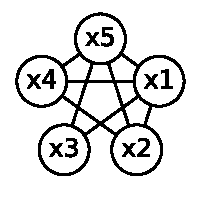
\includegraphics[width=\linewidth]{img/401a2e0bee9ea19714a37a3c2bfa4c78f5a92ea31c623ab3bc7826d5ed95c330.pdf}
			\vspace{-2em}
			\par\small (b)
		\end{minipage}
		\hfill
		\begin{minipage}{0.25\linewidth}
			\centering
			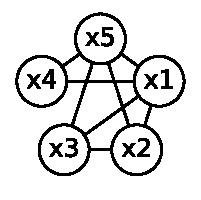
\includegraphics[width=\linewidth]{img/4b541ec99ee9b0f060e784c888fc378dca74b6d8ff80f5ccc8336615aca46695.pdf}
			\vspace{-2em}
			\par\small (c)
		\end{minipage}

		\begin{minipage}{0.25\linewidth}
			\centering
			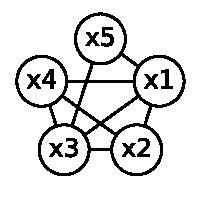
\includegraphics[width=\linewidth]{img/6eeebca324db75f7c0a719672bf306f79b5afe806b2a8814f0b2f2beedb3b891.pdf}
			\vspace{-2em}
			\par\small (d)
		\end{minipage}
		\hfill
		\begin{minipage}{0.25\linewidth}
			\centering
			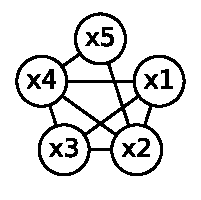
\includegraphics[width=\linewidth]{img/71f4c81555ee6516f44f4d05f5e6f67edd5de0ed42a1cdbcb2f2af72c3232b75.pdf}
			\vspace{-2em}
			\par\small (e)
		\end{minipage}
		\hfill
		\begin{minipage}{0.25\linewidth}
			\centering
			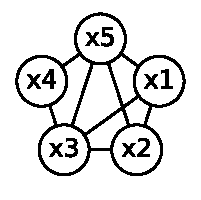
\includegraphics[width=\linewidth]{img/7d7c7231a399fc001d20da820222d60b8205b145c0e4fafd9cf2f3ebf1eec22d.pdf}
			\vspace{-2em}
			\par\small (f)
		\end{minipage}
		\captionof{figure}{Automorfisma Graf}
		\label{fig:contoh-automorfisma}
	\end{minipage}
\end{center}

Automorfisma graf adalah isomorfima suatu graf ke dirinya sendiri. Salah satu cara untuk menunjukkan automorfisma graf adalah menggunakan representasi kanonik. Hal ini telah dilakukan oleh \citeauthor{mckay2014} di \citeyear{mckay2014}. Jika dua graf memiliki representasi kanonik yang sama, maka kedua graf tersebut isomorfik. Sebaliknya, jika representasi kanonik berbeda, maka kedua graf tersebut tidak isomorfik.

Untuk graf tak berarah, representasi kanonik oleh \citeauthor{mckay2014} dituliskan dalam format \verb`graph6`. Sebagai ilustrasi, \autoref{fig:contoh-graf} memiliki representasi \verb`DV{` dalam format \verb`graph6`. Kemudian, setiap graf pada \autoref{fig:contoh-automorfisma}, dari (a) sampai (f), berturut-turut memiliki representasi \verb`D\{`, \verb`Du{`,  \verb`D{{`,  \verb`D~g`,  \verb`D~S`,  dan \verb`Dx{` dalam format \verb`graph6`. Akan tetapi, graf pada \autoref{fig:contoh-graf} dan semua graf pada \autoref{fig:contoh-automorfisma} memiliki representasi kanonik yang sama, yaitu \verb`DN{` dalam format \verb`graph6`, sehingga semuanya merupakan automorfisma dari graf yang sama.

\section{Dimensi Metrik}

Misalkan \(G\) adalah sebuah graf terhubung dengan himpunan simpul \(V = \{v_1, v_2, \ldots, v_n\}\), dan \(d(x, y)\) adalah jarak antara simpul \(x\) dan \(y\) di \(G\). Pilih sembarang \(W = \{w_1, w_2, \ldots, w_k\} \subseteq V\). Untuk \(v \in V\), tupel terurut
	\[ r(v|W) = (d(w_1, v), d(w_2, v), \ldots, d(w_k, v)) \]
adalah representasi dari \(v\) terhadap \(W\). Himpunan \(W\) adalah \foreign{resolving set}, atau himpunan pembeda, untuk \(G\) apabila
	\[ \forall u, v \in V, u \neq v \implies r(u|W) \neq r(v|W) \]
atau dengan kata lain, seluruh simpul dalam \(G\) memiliki representasi unik terhadap \(W\).

Dimensi metrik dari \(G\) adalah kardinalitas minimum dari himpunan pembeda untuk \(G\) \citep{tillquist2023}. Sebagai ilustrasi, ambil \autoref{fig:contoh-graf}. Coba \(W = \{x_2, x_4\}\).
\[
\begin{array}{ccccc}
	r(x_1|W) & = & ( d(x_2, x_1), \; d(x_4, x_1) ) & = & (2, 1) \\
	r(x_2|W) & = & ( d(x_2, x_2), \; d(x_4, x_2) ) & = & (0, 1) \\
	r(x_3|W) & = & ( d(x_2, x_3), \; d(x_4, x_3) ) & = & (2, 1) \\
	r(x_4|W) & = & ( d(x_2, x_4), \; d(x_4, x_4) ) & = & (1, 0) \\
	r(x_5|W) & = & ( d(x_2, x_5), \; d(x_4, x_5) ) & = & (1, 1)
\end{array}
\]
Ditemukan \(\{x_2, x_4\}\) bukanlah himpunan pembeda karena \(r(x_1|W) = r(x_3|W)\). Untuk \autoref{fig:contoh-graf}, tidak ada himpunan pembeda dengan kardinalitas 2. Dimensi metrik dari graf ini adalah 3, dengan contoh solusi \(\{x_1, x_4, x_5\}\), atau \(\{x_1, x_3, x_4\}\), dan himpunan pembeda lainnya yang berkardinalitas 3.

\section{Dimensi Metrik Sisi}

Misalkan \(G\) adalah sebuah graf terhubung dengan himpunan simpul \(V\), himpunan sisi \(E = \{e_1, e_2, \ldots, e_n\}\), dan \(d(x, y)\) adalah jarak antara simpul \(x\) dan \(y\) di \(G\). Untuk sembarang simpul \(z\) dan sembarang sisi \(e\) di \(G\), jika \(e\) adalah sisi yang menghubungkan simpul \(x\) dan \(y\), maka jarak dari \(z\) ke \(e\) adalah \( d(z, e) = \min(d(z, x), d(z, y)) \). Ambil sembarang \(W = \{w_1, w_2, \ldots, w_k\} \subseteq V\). Untuk \(e \in E\), tupel terurut
	\[ r(e|W) = (d(w_1, e), d(w_2, e), \ldots, d(w_k, e)) \]
adalah representasi dari \(e\) terhadap \(W\). Himpunan \(W\) adalah \foreign{edge resolving set}, atau himpunan pembeda sisi, untuk \(G\) apabila
	\[ \forall e, f \in E, e \neq f \implies r(e|W) \neq r(f|W) \]
atau dengan kata lain, seluruh sisi dalam \(G\) memiliki representasi unik terhadap \(W\).

Dimensi metrik sisi dari \(G\) adalah kardinalitas minimum dari himpunan pembeda sisi untuk \(G\) \citep{kelenc2018}. Sebagai ilustrasi, ambil \autoref{fig:contoh-graf}. Coba \(W = \{x_1, x_4, x_5\}\).
\[
\begin{array}{ccccc}
	r(e_1|W) & = & ( d(x_1, e_1), \; d(x_4, e_1), \; d(x_5, e_1) ) & = & (0, 1, 1) \\
	r(e_2|W) & = & ( d(x_1, e_2), \; d(x_4, e_2), \; d(x_5, e_2) ) & = & (0, 0, 1) \\
	r(e_3|W) & = & ( d(x_1, e_3), \; d(x_4, e_3), \; d(x_5, e_3) ) & = & (0, 1, 0) \\
	r(e_4|W) & = & ( d(x_1, e_4), \; d(x_4, e_4), \; d(x_5, e_4) ) & = & (1, 0, 1) \\
	r(e_5|W) & = & ( d(x_1, e_5), \; d(x_4, e_5), \; d(x_5, e_5) ) & = & (1, 1, 0) \\
	r(e_6|W) & = & ( d(x_1, e_6), \; d(x_4, e_6), \; d(x_5, e_6) ) & = & (1, 0, 1) \\
	r(e_7|W) & = & ( d(x_1, e_7), \; d(x_4, e_7), \; d(x_5, e_7) ) & = & (1, 1, 0) \\
	r(e_8|W) & = & ( d(x_1, e_8), \; d(x_4, e_8), \; d(x_5, e_8) ) & = & (1, 0, 0)
\end{array}
\]
Ditemukan \(\{x_1, x_4, x_5\}\) bukanlah himpunan pembeda sisi karena \(r(e_4|W) = r(e_6|W)\). Untuk \autoref{fig:contoh-graf}, tidak ada himpunan pembeda sisi dengan kardinalitas 3. Dimensi metrik sisi dari graf ini adalah 4, dengan contoh solusi \(\{x_1, x_2, x_3, x_4\}\), atau \(\{x_1, x_2, x_3, x_5\}\), dan himpunan pembeda sisi lainnya yang berkardinalitas 4.

\section{\foreign{Satisfiability Modulo Theories}}

SMT, atau \foreign{satisfiability modulo theories}, secara umum adalah proses mencari nilai dari variabel-variabel dalam ekspresi matematika yang menyebabkan ekspresi tersebut menjadi benar. Jika suatu solusi ada, ekspresi tersebut terbilang \foreign{satisfiable}. Jika solusi tidak ada, ekspresi tersebut terbilang \foreign{unsatisfiable}. Proses ini tidak menentukan solusi mana yang akan diberikan, melainkan hanya mencari satu solusi apa pun, yang kemudian disebut sebagai \foreign{model}.

Istilah \foreign{modulo theories} merujuk pada penggunaan teori tertentu, seperti aritmetika bilangan bulat, bilangan riil, \foreign{array}, atau \foreign{bit-vectors}. Pemilihan teori biasanya disesuaikan dengan tujuan pemodelan. Bergantung pada apakah suatu permasalahan ingin ditunjukkan sebagai \foreign{satisfiable} atau \foreign{unsatisfiable}, teori yang digunakan dapat pula berbeda untuk memfasilitasi pemanfaatan sifat-sifat permasalahan tersebut agar lebih ramah terhadap komputasi.

\foreign{Solver} adalah program yang mengimplementasikan proses dari SMT, mengevaluasi ekspresi, dan dapat menghasilkan model. Secara komputasi, \foreign{solver} mungkin untuk tidak menunjukkan hasil, bergantung pada konfigurasi seperti batas waktu eksekusi, maupun dari keterbatasan implementasi teori.

Penjelasan lebih lengkap mengenai SMT dapat ditemukan pada \cite{barrett2018}.

\subsection{\foreign{Boolean Satisfiability}}

\foreign{Boolean satisfiability} dalam SMT adalah teori yang memuat variabel boolean dan operasi boolean pada umumnya \citep{yurichev}. Sebagai ilustrasi, dapat diperhatikan ekspresi
	\[ (x_1 \land x_2) \lor (x_1 \land x_3) \]
dengan \(x_1, x_2, x_3\) adalah variabel boolean. Tabel kebenaran untuk ekspresi tersebut dapat dikonstruksi seperti berikut:
\vspace{-0.5em}
\[
\begin{array}{cccc}
	x_1 & x_2 & x_3 & (x_1 \land x_2) \lor (x_1 \land x_3) \\ [4pt]
	\False & \False & \False & \False \\
	 \True & \False & \False & \False \\
	\False &  \True & \False & \False \\
	 \True &  \True & \False &  \True \\
	\False & \False &  \True & \False \\
	 \True & \False &  \True &  \True \\
	\False &  \True &  \True & \False \\
	 \True &  \True &  \True &  \True
\end{array}
\]

\noindent Oleh karena itu, salah satu \foreign{model} yang dapat dihasilkan oleh \foreign{solver} adalah \(x_1 = \True, x_2 = \False, x_3 = \True\).

Dalam \foreign{boolean satisfiability}, terdapat pula batasan \(\mathrm{AtLeast}\) dan \(\mathrm{AtMost}\) untuk menentukan paling sedikit dan paling banyak variabel yang boleh bernilai benar. Misalnya, dengan menambahkan batasan \(\mathrm{AtLeast}(3)\) ke contoh sebelumnya, \(x_1 = \True, x_2 = \False, x_3 = \True\) tidaklah lagi solusi yang sah.

\subsection{\foreign{Pseudo Boolean}}

\foreign{Pseudo boolean} adalah ekstensi dari teori \foreign{boolean satisfiability} yang dapat menyatakan bentuk ekspresi linear dengan koefisien bilangan bulat atas variabel boolean \citep{yurichev}. Teori ini mendukung tiga operasi relasi, yaitu:
\[
\begin{array}{lcl}
	a_1 x_1 + a_2 x_2 + \ldots + a_i x_i &\leq& a \\
	b_1 x_1 + b_2 x_2 + \ldots + b_j x_j &=& b \\
	c_1 x_1 + c_2 x_2 + \ldots + c_k x_k &\geq& c \\
\end{array}
\]
di mana \(a, a_1, \ldots, a_i, b, b_1, \ldots, b_j, c, c_1, \ldots, c_k\) adalah konstanta \foreign{integer} (bilangan bulat), dan \(x_1,\ldots,x_i,x_j,x_k\) adalah variabel boolean. Ketika variabel boolean bernilai benar, perkaliannya dengan konstanta menjadi seperti perkalian dengan angka 1. Ketika variabel boolean bernilai salah, perkaliannya dengan konstanta menjadi seperti perkalian dengan angka 0. Ambil contoh berikut:
\[
\begin{array}{rcl}
	x_1 + x_2 + x_3 + x_4 &=& 2 \\
	x_1 + x_2 &\leq& 1 \\
	x_3 + x_4 &\leq& 1
\end{array}
\]
dengan \(x_1, x_2, x_3, x_4\) adalah variabel boolean. Ekspresi ini memiliki seluruh konstantanya yang sama dengan 1. Salah satu \foreign{model} yang dapat dihasilkan oleh \foreign{solver} adalah \(x_1 = \True, x_2 = \False, x_3 = \True, x_4 = \False\).

\subsection{\foreign{Linear Integer Arithmetic}}

\foreign{Linear integer arithmetic}, atau LIA, dalam SMT adalah teori yang memuat variabel \foreign{integer}, atau bilangan bulat, dan operasi \foreign{integer} pada umumnya \citep{yurichev}. Contoh \foreign{pseudo boolean} sebelumnya dapat dinyatakan ulang dalam bentuk LIA.
\[
\begin{array}{rcl}
	x_1 + x_2 + x_3 + x_4 &=& 2 \\
	x_1 + x_2 &\leq& 1 \\
	x_3 + x_4 &\leq& 1
\end{array}
\]
\[ 0 \leq x_1 \leq 1, \quad 0 \leq x_2 \leq 1, \quad 0 \leq x_3 \leq 1, \quad 0 \leq x_4 \leq 1 \]
dengan \(x_1, x_2, x_3, x_4\) adalah variabel \foreign{integer}. \foreign{Model} yang dapat dihasilkan oleh \foreign{solver} yang mirip dengan hasil dari \foreign{pseudo boolean} sebelumnya adalah \(x_1 = 1, x_2 = 0, x_3 = 1, x_4 = 0\).

\section{Z3}

Z3 adalah salah satu dari banyak \foreign{solver} SMT yang ada. Z3 dikembangkan oleh Microsoft Research dan dirancang khusus untuk menyelesaikan formula logika dari berbagai macam jenis teori. Z3 merupakan \foreign{solver} modular, dengan menggunakan arsitektur DPLL(T), menggabungkan berbagai prosedur untuk teori-teori yang berbeda \citep{demoura2008}.

Dibandingkan dengan \foreign{solver} lain yang hanya mengkhususkan diri pada teori-teori tertentu, Z3 mendukung kombinasi teori yang lebih kompleks . Selain itu, Z3 juga mendukung penyelesaian inkremental, generasi bukti (\foreign{proof generation}), ekstraksi \foreign{unsat core}, serta penggunaan kuantor (universal dan eksistensial) \citep{bjorner}.

Perlu dipahami bahwa Z3, maupun SMT \foreign{solver} pada umumnya, tidak melakukan manipulasi simbolik sebagaimana \foreign{computer algebra system} (CAS). SMT \foreign{solver} difokuskan pada penentuan \foreign{satifiability} suatu ekspresi menggunakan prosedur seperti DPLL(T) \citep{demoura2008, bjorner}. Sebaliknya, CAS dirancang untuk manipulasi simbolik seperti penyederhanaan ekspresi, integrasi, atau diferensiasi simbolik \citep{geddes1992}. Oleh karena itu, SMT \foreign{solver} dan CAS merupakan kelas asisten komputasi yang berbeda.
